\documentclass[letterpaper,11pt]{article}
\usepackage[margin=1.1in]{geometry}
\usepackage{amsmath}
\usepackage{enumitem}
\usepackage[utf8]{inputenc}
\usepackage{pmboxdraw}
\usepackage{verbatim} % for verbatim environment and \verbatiminput
\usepackage{sverb} % for \verbinput
\usepackage{verbatimbox}
\usepackage{algorithm}
\usepackage{algorithmic}


% For angular brackets
\usepackage{textcomp}
% Skip the indents for every paragraph
\usepackage{parskip}
\usepackage{epsfig,endnotes}
\usepackage[T1]{fontenc}
\usepackage{times}
\usepackage[square,comma,numbers,sort&compress]{natbib}
\usepackage[breaklinks,colorlinks]{hyperref}
\hypersetup{citecolor=blue,linkcolor=blue}
\usepackage{listings}
%\usepackage[outputdir=latex.out]{minted}
\usepackage{endnotes,graphicx,fancyvrb,multirow}
\usepackage{booktabs}
\usepackage{underscore}
\usepackage{amssymb}
\usepackage{tikz}
\usetikzlibrary{shapes,arrows,shadows,matrix,positioning,fit}


\newcommand\todo[1]{\textcolor{red}{TODO: #1}}
\newcommand\note[1]{\textcolor{red}{NOTE: #1}}

\newcommand\ic[1]{\texttt{#1}}
\newcommand\red[1]{\textcolor{red}{#1}}

\newcommand\para[1]{\vspace*{5pt} \noindent \textbf{#1}}
\newcommand\TODO{\textcolor{red}{TODO}}

\newenvironment{code}
{\begin{center}
	\fontfamily{pcr} \selectfont
    \begin{tabular}{|p{0.9\textwidth}|}
    \hline
	\\[-8pt]
    }
    {
	\\[-8pt]
	\\
	\hline
    \end{tabular}
    \end{center}
}


\newenvironment{temporary}{\par\color{blue}}{\par}


\newcommand{\squishenumerate}{
   \begin{enumerate}
    { \setlength{\itemsep}{0pt}      \setlength{\parsep}{3pt}
      \setlength{\topsep}{3pt}       \setlength{\partopsep}{0pt}
      \setlength{\leftmargin}{2em} \setlength{\labelwidth}{1em}
      \setlength{\labelsep}{0.5em} } }

\newcommand{\squishenumerateend}{
    \end{enumerate}  }

\newcommand{\squishlist}{
   \begin{list}{$\bullet$}
    { \setlength{\itemsep}{0pt}      \setlength{\parsep}{3pt}
      \setlength{\topsep}{3pt}       \setlength{\partopsep}{0pt}
      \setlength{\leftmargin}{2em} \setlength{\labelwidth}{1em}
      \setlength{\labelsep}{0.5em} } }

\newcommand{\squishlisttwo}{
   \begin{list}{$\bullet$}
    { \setlength{\itemsep}{0pt}    \setlength{\parsep}{0pt}
      \setlength{\topsep}{0pt}     \setlength{\partopsep}{0pt}
      \setlength{\leftmargin}{2em} \setlength{\labelwidth}{1.5em}
      \setlength{\labelsep}{0.5em} } }

\newcommand{\squishend}{
    \end{list}  }
    

\newcommand{\enablecomments}{0}

\ifnum\enablecomments=1
  \newcommand{\congyu}[1]{\textcolor{blue}{\textbf{CL: #1}}}
  \newcommand{\paul}[1]{\textcolor{purple}{\textbf{PN: #1}}}
  \newcommand{\yi}[1]{\textcolor{orange}{\textbf{YS: #1}}}
  \newcommand\pf[1]{\textcolor{red}{PF: #1}}
\else
  \newcommand{\congyu}[1]{}
  \newcommand{\paul}[1]{}
  \newcommand{\yi}[1]{}
  \newcommand\pf[1]{}
\fi
 
\graphicspath{ {./imgs/} }
\usepackage[export]{adjustbox}
\usepackage{caption} 
\captionsetup[table]{skip=2pt}


\begin{document}

\begin{center}
    {\LARGE{Lab 2: Greybox Mutation-based Testing (Fuzzing)}}\\
	\vspace*{10pt}
	{\Large{CS408, Spring 2026}}\\
    \vspace*{10pt}

  {\large{\textbf{Group Project (150 points)\\
        Due date: March 23, 2026}}}\\
      \vspace*{15pt}
      \textbf{Lead TA}: Ruixin Wang (\href{mailto:ruixinw@purdue.edu}{ruixinw@purdue.edu})
\end{center}

%\todo{Add an option to make the framework print the test case that causes a failure.}

%\todo{Improve the skeleton.}

%\todo{Create a C version of the skeleton.}



% \todo{Update github classroom link}

% \pf{Integrate the changes from the Ed FAQ mega-thread.}

% \pf{Change the targets.}

% \pf{Propose more improvements to the lab.}

% \pf{Make the handout consistent with the Lab 1 handout.}

% \pf{Integrate the change log changes in Section 12.}

% \pf{Check that the instruction in the setup section are correct}


\section{Project Description}

In this project, you will build a basic greybox fuzzer from scratch.
You will start with building a blackbox fuzzer, then turn it into a greybox fuzzer.
You will also enhance your fuzzer with grammar-based input generation and mutation.
You will evaluate your fuzzer with the fuzzing targets we assign.
As the last task of this project, you will get hands-on experience with AFL, a well-known, state-of-the-art greybox fuzzer.

% The fuzzing targets are JSON, YAML and XML parsing libraries.
% Each group will be assigned two targets, one from XML libraries and one from either JSON or YAML libraries.
% The target assignment will be announced in Edstem.
% The tarballs of all fuzzing targets are provided in the skeleton code directory.
% Please make sure you are always using the target code provided by us.

The fuzzing targets are JSON (\href{https://github.com/kgabis/parson}{parson}) and YAML (\href{https://github.com/pantoniou/libfyaml/tree/master}{libfyaml}) parsing libraries.
The tarballs of these fuzzing targets are provided in the skeleton code directory.
Please make sure you are always using the target code provided by us.

% \pf{I think we should specify the targets in the handout and make everyone test the same. This will simplify things. }
% \congyu{done}


Here is the breakdown of points for this lab assignment:

\begin{itemize}
    \item \textbf{Fuzzing framework implementation (130 points)}:  Points are awarded based on the framework's effectiveness. We will run several validation tests to check the basic functionality of your fuzzer.
    
    \item \textbf{Using AFL (10 points)}: Points are awarded based on the environment (e.g., script) you provide for us to run AFL.
    
    \item \textbf{Report (10 points)}: Points are awarded based on whether your report contains the required analysis and results. \textit{You must answer all the questions listed in the handout.}
    
    \item \textbf{Fuzzer competition (5 bonus points)}: Bonus points are awarded based on your fuzzer performance relative to your peers, particularly in terms of bug-finding efficiency and effectiveness. Only the top performing projects will be awarded full or partial bonus points. 
    % \pf{Need to have a section talking about this? How should they design their tools to increase their chances (i.e., what is performance in this case)?}
    % \congyu{I added a section at the end}
\end{itemize}


% The fuzzing framework you will implement is worth 80 points.
% Blackbox fuzzing functionality worth 30 points.
% greybox fuzzing functionality worth 30 points.
% Grammar-based generation functionality worth 20 points.
% AFL is worth 10 points.
% Blackbox fuzzing functionality worth 30 points, which includes implementing the  fuzzer-harness IPC interfacae (15 points) and the ability to mutate from given seeds (15 points).
% greybox fuzzing functionality worth 30 points, which includes the ability to correctly report the code coverage of each input in the corpus (15 points), the fuzzer-harness IPC interface with coverage support (5 points), the ability to minimize the input (10 points).
% Grammar-based generation functionality worth 30 points. The mutation and generation fucntionality worth 15 points.
% The remaining 10 points are assigned based on the report you will submit. 
% We will run several tests to validate the functionality of your fuzzer.
% We will also evaluate your fuzzer on several secret vulnerable binaries. 
% \pf{Can we make it more than one secrete binary, it becomes too luck-dependent with just one binary} 
% \congyu{Yes. We can.}
% 5 extra bonus points will be assigned based on how effective your fuzzer is on the secrect vulnerable binary (e.g., how many bugs your fuzzer can discover).
% You can earn a total of 5 bonus points based upon your class ranking (e.g., bug finding efficiency/effectiveness).
% A more detailed point breakdown is listed in the rest of the handout.

% \pf{The way we explain the points is too confusing, making a bullet list to explain more clearly}
% \congyu{done}

Read the assignment \textbf{entirely} before starting any work on it.

This is a group project –- only collaboration between pre-registered group members is allowed.

\fbox{
\begin{minipage}{\textwidth}
\textbf{REQUIREMENT:}
You are required to submit original code that you or your group members have written for this lab.
Using code from online sources or other people is strictly
prohibited. Violations of this policy may result in disciplinary action,
including but not limited to zero points for this lab, academic probation, or
other consequences as determined by the academic integrity guidelines of our
institution/course.
\end{minipage}
}

% \pf{Need to add a more explicit disclaimer about which code they can use in
% their labs (e.g., they can only submit code written by themselves.); this is
% important because they may be tempted to use online code in this lab.} \congyu{added}

% \pf{Run a spell and grammar checker ASAP.} \congyu{done}


\section{Project Setup and Development Workflow}

Please follow the instructions in \autoref{sec:appx:setup} to \textbf{clone}, \textbf{setup}, and regularly \textbf{update} your GitHub classroom private repository.

\fbox{
\begin{minipage}{\textwidth}
\textbf{REQUIREMENT:} Your private GitHub classroom repository is going to be used to: (a) help staff provide support to students when there are questions about their project, (b) help students backup and cooperate within the group, (c) investigate cases of plagiarism, and (d) investigate cases of uneven contributions among group members.
Hence, in this course, students are \textbf{required} to use GitHub Classroom and regularly commit and push their updates (e.g., approximately every 2 hours of work). Not following this requirement will lead to \textbf{partial or total loss of points} in the final grade of the project.
\end{minipage}
}


\section{Fuzzing Background}

Fuzzing is a dynamic software testing technique that is very effective at discovering bugs (and security vulnerabilities).
The basic idea of fuzzing is straightforward: during testing, a fuzzer keeps
generating random input, feeding it to the system under test (SUT), and checking
if the input causes the program to fail (e.g., crashes).
The term \textit{fuzzing} dates back to the 1990s, when B. P. Miller et al.~[1] built a random input generator to test 90 UNIX programs and successfully crashed 24 of them.
This marks the dawn of this effective testing technique.
Nowadays, fuzzing has been widely used in testing various software, ranging from simple libraries to complex system software such as Linux kernel~[2].
Some modern languages such as Golang, have native support for fuzzing~[3] that allows push-button testing.

During testing, some fuzzing techniques collect \textit{internal information} from the SUT.
Note that the term internal information here does not refer to the explicit output of a SUT, such as the return code or console output, but rather the internal state of the SUT when it executes with a test input, such as code coverage.
Such information reflects how well a test input exercises the SUT, and thus can serve as valuable feedback to a fuzzer on how good a test input is, or even inform a fuzzer of the potential strategies to generate better input.
Intuitively, the more information a fuzzer can collect from the SUT, the better input it can generate.
Unfortunately, collecting more information comes at a cost: it usually relies on
techniques (e.g., compiler instrumentation, software emulation, or
interpretation) that might drastically degrade the testing throughput and may
harm the effectiveness of a fuzzer. In short, there is a trade-off between the
test input quality and testing throughput.

In general, based on the amount of internal information a fuzzer collects, there are three types of fuzzing techniques: blackbox fuzzing, greybox fuzzing, and white-box fuzzing.
Blackbox fuzzing does not collect any internal information from SUT and it blindly generates test input.
Greybox fuzzing stands in the middle and collects basic internal information such as code coverage.
White-box fuzzing, in contrast, collects all internal information from SUT (e.g., using symbolic execution).
As a result, greybox fuzzing balances the test input quality and testing throughput, and often scales better than the other two approaches.

% \pf{Change "see" to "collect".} \congyu{done}

% \textbf{TODO: move points to sections}

% \textbf{TODO: move the lab1 warnings from lab1}

% \textbf{TODO: add a competition for 5 points.}

% The remaining points (20 points) and 10 extra points will be assigned depending on the effectiveness of your
% framework and test suit at finding an additional set of injected bugs that are not provided to you.
% Hence, you should ensure that your framework is effective at triggering and detecting a wide-range of bugs.

% [TODO: emphasis that this lab is open: students can try different heuristics freely ]


% Your project will be graded largely based on the report you submitted. In the report, you need to answer the questions listed in the handout. The report should also include your design and provide the reasons for going for certain choices.

% You also need to submit your project code. [TODO: requirement on directory structure] We will first test your fuzzer using the same targets you are assigned. [TODO: provide details on how we grade this] We will also run your fuzzer on a different target. If your fuzzer can discover the vulnerabilities we injected, you will get bonus points. [TODO: maybe provide hint about the target?]

\section{Fuzzer User Interface}

\subsection{Command Line Interface}

Your fuzzer should implement the following command line interface:

\begin{verbatim}
$ python fuzzer.py -o <output_dir> [-i <seed_dir>] [-g <grammar_file>]
[--greybox] [--dict] [--competition] <harness>
\end{verbatim}


where:

\begin{itemize}
    \item \textbf{\texttt{-o}}: the path to the output directory.
    \begin{itemize}
        \item If the output directory does not exist, the fuzzer creates it, \textit{including all necessary parent and ancestor directories}. This can be achieved using \texttt{os.makedirs}.
        \item If the output directory exists or the fuzzer cannot create a new directory, the fuzzer reports an error and exits with code 1.
        \item The output directory includes certain sub-directories or files, which will be described later in the handout. You must strictly follow the requirements specified in the handout.
    \end{itemize}
    \item \textbf{\texttt{-i}}: an optional parameter that specifies the path to a seed directory. If the seed directory does not exist, the fuzzer reports an error and exits with code 1. This parameter has no effect when a grammar file is specified.
    \item \textbf{\texttt{-g}}: an optional parameter that specifies the path to an input grammar file (see \autoref{sec:grammar}).
    \item \textbf{\texttt{{-}{-}greybox}}: an optional parameter that switches the fuzzer to greybox fuzzing mode (see \autoref{sec:greybox}). The fuzzer operates in blackbox mode by default.
    \item \textbf{\texttt{{-}{-}dict}}: an optional parameter that enables the dictionary feature (see \autoref{sec:dictionary}). This allows the fuzzer to use a predefined set of inputs to guide its exploration.
    \item \textbf{\texttt{{-}{-}competition}}: an optional parameter that will be passed when we test your fuzzer for bonus points. Your fuzzer should enable the enhanced features (if implemented) under this mode (\autoref{sec:fuzzercompetition}).
    % \pf{Need to explain this in a Section. Are they allowed to parallelize tests?} \congyu{added a section at the end. they can parallelize} \paul{Added ref to section}    \item \textbf{\texttt{<harness>}}: the path to a fuzzing harness.
    \item \textbf{\texttt{<harness>}}: the path to a fuzzing harness.
\end{itemize}

Your fuzzer should be able to be terminated using Ctrl-C.

\textbf{Please make sure relative paths work with your fuzzer}!

\subsection{Console Output}

Your fuzzer needs to print a line of its state every 5 seconds in the following format:

\begin{verbatim}
duration=[hour]h[minute]m[second]s, exec=[#executions], 
corpus=[#corpus], coverage=[covered]([total]),
bugs=[#unique]([#total])
\end{verbatim}

For example, the following line

\begin{verbatim}
duration=0h10m23s, exec=334, corpus=4, coverage=22(345), bugs=1(3)
\end{verbatim}

means the fuzzer has run for 10 minutes and 23 seconds; it has executed 334 input; its corpus size is 4 (in blackbox fuzzing this is always 0 as there is no corpus); it has covered 22 edges out of 345 edges in total (in blackbox this is 0 as we don't have the edge count of the CFG for the binary generated as there was no compiler instrumentation); it has triggered 1 unique bug (defined in \autoref{subsec:bug}) and 3 bugs in total.

% \pf{"bugs" means failed executions? Need to clarify this.} \yi{Bugs means "crash" or "hung". Congyu talks about it in later sections.}
% \paul{done. added ref}
% \paul{Removed deduplicated and make use of ref to subsec:bug instead}
% \pf{Congyu, is this handled. If so, please comment it.}


% By default, the fuzzer runs in blackbox mode.
% -i specifies the path to a seed directory.
% If this directory does not exist, your fuzzer should report error and exit with code 1.
% -o specifies the path to the output directory.
% If this directory exists, your fuzzer should report error and exit with code 1.
% Otherwise, it will create the specified directory along with all necessary parent and ancestor directories if they do not exist (you can make use of os.makedirs).
% The output directory contains certian sub-directories or files that will be described in the rest of the handout.
% \texttt{-}\texttt{-}greybox is an optional parameter, which specifies that the fuzzer runs in greybox fuzzing mode (\autoref{sec:greybox}).
% -g is an optional parameter, which specifies the path to an input grammar file (\autoref{sec:grammar}).
% When a grammar file is specified, the fuzzer will switch to using grammar-based input generation.

% \pf{Write this text above in a bullet list. This is too confusing as is.} \congyu{done}

\section{Task 1: Blackbox Fuzzing (30 Points)}
\label{sec:blackbox}

% \yi{I changed the title to be Task 1.... If this is what you mean when refering to task 1, please change the rest titles similarly}
% \congyu{done}

% \yi{I added the following description to the task. Please modify it if needed.}
% \congyu{}

In this task, you will implement a blackbox fuzzer.
It takes a set of known input, seeds, and a harness program, which feeds seeds to the SUT, and executes the seed on the SUT.
Seeds are initial test inputs that can exercise code paths that are difficult for a fuzzer to generate on its own.
Then, these seeds are further mutated via various means in an attempt to trigger more diverse behaviors in the SUT.
Once a bug (\autoref{subsec:bug}) is triggered by a certain input, your fuzzer will generate a bug report. The detailed requirements of each component of the blackbox fuzzer are described in the following sections.

Seeds are used rather than random input as it is improbable that a good seed is generated at random.
For instance, in the case of JSON, it would be hard to generate a file that has a correct set of matching parentheses that fit the syntax.
Furthermore, the mutations applied are on a small scale to maximize the chance of creating more valid input.

% \subsection{Seeds}
% Fuzzers typically require a set of \textit{seeds} as input. Seeds are initial test inputs.
% The seeds are usually inputs that can exercise code paths that are difficult for a fuzzer to generate on its own.
% For example, imagine a JSON parser library that takes a string as input and returns a parsed data structure.
% The library would reject the input at a very early stage if the input is not syntactically correct (e.g., parentheses do not match). 
% If a fuzzer simply generates random bytes as input, it cannot exercise enough code paths in a short time since most of them will get rejected easily.
% Given initial seeds, a fuzzer can generate new input by mutating them and creating diverse input that can potentially reach deeper into the code.

% \pf{Students may get confused with this section: where is the task? Need to have here or somewhere at the top of section 5 some high-level explanation of their tasks.} \pf{I would have expected the most basic tasks is for them to implement a mechanism that just runs the target with some input and figures out if it crashed or not; think about whether the current order of tasks/text makes sense.}
% \paul{done. Folded into some background information without a section name.}

\subsection{Mutation}
In this task, your fuzzer generates an input by randomly selecting a seed and mutating it.
Make sure that the mutation always produces either printable ASCII characters (value from 32 to 126), spaces, newlines, or tabs.
Note that one should refrain from creating a null character as it truncates the seed and is likely to make it invalid.
You need to implement the following mutators:
\begin{enumerate}
    \item \textbf{insert:} insert a random byte at a random place
    \item \textbf{delete:} delete a random byte at a random place
    \item \textbf{flip:} randomly pick a byte to change it to another random byte
    % \item \textbf{arith:} randomly pick a byte and randomly add or subtract it by a random number in the $[1, 8]$ range. This range is a heuristic used in AFL to transmute a character of one type into another (eg. number -> number or capital letter -> capital letter). Make sure that the mutation always produces printable ASCII characters. \pf{how should they make sure this happens?} However, one should refrain   from creating a null character as it truncates the seed and is likely to make it invalid. 
    % \pf{Last sentence is also unclear what is the algorithm they should implement?}
    % \congyu{I remove this mutator. It would involve so many corner cases}
    % \item \textbf{arith:} randomly pick a byte and randomly add or subtract it by a random number in $[1, 8]$. 
    % % This range is a heuristic used in AFL to transmute a character of one type into another (eg. number -> number or capital letter -> capital letter).
\end{enumerate}

Your fuzzer should pick between 1 to 16 random mutators, out of the list of 3 mutator types, to apply to a randomly picked seed. 
% You are welcome to implement more different mutators!

% \pf{They should be required to print information about which mutations they are applying on each mutation. I.e., we should specify their algorithm fully 
% (except for the competition mode).}
% \congyu{Ask them to save more information in 5.4.}
% \congyu{Hmmm I think we have specified the algorithm?}
% \pf{We're telling them that they can come up with their own, and we're not saying clearly the distribution. (There might be other things that we're not saying explicitly that could be important too.)}
% \pf{We can ask them to come up with their own for the competition mode though, but I would suggest we ask them to activate this mode with a special command line flag.}
% \congyu{done}


% [TODO: mention entropy but we just used fixed ones]
% [TODO: put an algorithm]

% \pf{Congyu, remove the points in the subsections. It's too fine-grained
% information to give the students about the grading, and we may need to adjust
% depending on how the lab goes.} \congyu{done (I removed the ones in subsections but not sections)}


\subsection{Harness}

% \textbf{[TODO: define the interface with more details; Complete after implementing the skeleton code]}

% \paul{Why s the input only 4 bytes?}
% \congyu{the length integet is 4 bytes. Clarified.}
% \paul{What is the 1 byte written to the egress pipe?}
% \congyu{mark the end of a execution. Clarified.}

% \textbf{Please make sure you implement the interface as follows. Otherwise, you will lose points.}


A fuzzing harness bridges the fuzzer and the fuzzing target (e.g., libraries). This is particularly important when the fuzzing target is a library, which can only be executed when linked with an application.
Specifically, a fuzzing harness takes the input from the fuzzer and feeds it to the fuzzing target.
In greybox fuzzing, it will also report the internal execution information to the fuzzer (see \autoref{sec:greybox}).

In blackbox fuzzing, the fuzzing harness will read the input from the \texttt{stdin}, execute the target with the given input, and then exit.
For example, to test the JSON library, you can pass the input JSON string to the parsing function.
Some JSON libraries also provide serialization functions, so you can call them to serialize the results of the parsing function, to easily test more code.
% \pf{Execute what?} \congyu{input; fixed} \pf{The input is not executable. Use "execute the target with the input given"?} \yi{fixed}
For each input, the fuzzer will spawn a harness process, write the input to the \texttt{stdin} of the harness process, and then wait for the harness process to exit.
\autoref{tab:blackboxfuzzerharness} illustrates this process.

% The harness runs in an infinite loop.
% At the beginning of each iteration, the harness waits on an ingress pipe.
% The fuzzer will first write a 4-byte integer into the pipe, which specifies the input length.
% The fuzzer will then write the input into the pipe.
% The harness will first read the input length, which helps it determine how many input bytes it should wait.
% Then it read the input.
% After the input is executed, the harness will inform the fuzzer by writing one byte to an egress pipe, then go to the next iteration.
% This byte only serves as a signal to inform the end of an execution.

% The fuzzer will generate and send the next input after it receives a byte from the pipe.

% A fuzzing harness is a program you implement that takes the input from the fuzzer and feeds it to the fuzzing target.
% The fuzzing harness you implemented will communicate with the fuzzer using two pipes.
% The harness runs in an infinite loop.
% At the beginning of each iteration, the harness waits on an ingress pipe.
% The fuzzer will first write a 4-byte integer into the pipe, which specifies the input length.
% The fuzzer will then write the input into the pipe.
% The harness will first read the input length, which helps it determine how many input bytes it should wait.
% Then it read the input.
% After the input is executed, the harness will inform the fuzzer by writing one byte to an egress pipe, then go to the next iteration.
% This byte only serves as a signal to inform the end of an execution.

% The fuzzer will generate and send the next input after it receives a byte from the pipe.


\begin{table}[ht]
\centering
\caption{Blackbox fuzzer harness workflow (time flows downwards)}
\label{tab:blackboxfuzzerharness}
\begin{tabular}{ll}
\toprule
\textbf{Blackbox Fuzzer}          & \textbf{Harness}       \\ \midrule
Spawn harness            &      \\
Write input               &  Wait on \texttt{stdin}    \\
Wait for the harness to exit          & Read input from \texttt{stdin}   \\
                    & Execute the input    \\
                     &  Exit                    \\ 
Timeout/Check exit status                      &                     \\ 
\bottomrule

\end{tabular}
\end{table}

% \pf{Need to be more specific about what they need to do here. Are we providing some code? We need to explain how what they are requested 
% to do related wot the code provided.}
% \congyu{Add a table. Simplify the process. No code is provided since this part is easy.}
% [TODO: more details on how harness setup pipes, e.g., using dup2()...]

\subsection{Bug Detection}
\label{subsec:bug}

Your fuzzer must be able to detect two types of bugs: crash and hung bugs.
Note that, if the target function returns an error code, it is not considered a bug.
Your fuzzer needs to monitor the exit code of the harness to detect any crashes.
Your fuzzer detects a hung situation when an execution spends more than 5 seconds (and needs to be terminated by your fuzzer).
Upon detecting a bug, the fuzzer should collect the combined standard output (\texttt{stdout}) and standard error (\texttt{stderr}) from the harness.
Then the fuzzer might need to generate a bug report.
 Here are the requirements:
\begin{itemize}
    \item \textbf{Deduplicate Based on Output:} To minimize duplicate bug reports, your fuzzer should deduplicate bugs based on the harness output. If two bugs generate the same output, they should be considered duplicates and not reported separately. Every failed execution that produces no output is considered a distinct bug. 
    %\pf{Consider saying something like: Every failed execution that produces no output is considered a distinct bug.} \congyu{done}
    \item \textbf{Assign Unique Bug IDs:} Each bug is assigned a unique ID, starting from 0. This ID is monotonically increasing as more bugs are found by your fuzzer. Note, this value should be set to 0 every time your fuzzer starts.
    %\pf{Does this counter reset every time the fuzzer process restarts. Or is this a persistent counter?} \congyu{we don't support checkpoint, i.e., every time the fuzzer starts freshly. so it always starts 0} \paul{done. added clarification.}

    \item \textbf{Bug Report Naming:} For bug $\#i$, the bug reports are saved into a directory named \texttt{i} within the \texttt{[output\_dir]/bugs} directory. Each bug directory contains the following files: 
    \begin{itemize}
        \item \textbf{input:} The input that caused the bug. For instance a JSON file's contents.
        \item \textbf{out:} The output from the harness.
        \item \textbf{prev:} The file name of the seed from which this input was mutated on a single line in the file (eg. "1").
        \item \textbf{mut:} The sequence of mutators used to generate this input. List each name (e.g., "insert") at a separate line.
        \item \textbf{type:} Type of the bug. Either "crash" or "hung" on a single line in the file.
    \end{itemize}
\end{itemize}

 The following is an example of a valid folder structure used to store output:

 \VerbatimInput{outputdir.c}
 
% \yi{suggested changes. mut: The sequence of mutators used to generate this input. List each name (e.g., "insert") at a seperate line.}
% \congyu{done}

% \yi{suggested changes. type: Type of the bug. Either "crash" or "hung"}
% \congyu{done}


% The fuzzer needs to monitor the exit status of the harness.
% It should report a bug if the harness crashes.
% Once a bug is found, the fuzzer needs to collect the output (combining the stderr and stdout) of the harness.
% The fuzzer needs to save both the input and output of the harness into the bug report directory, which is a directory named 'bugs' under the output directory.
% Each bug is assigned a unique bug ID, which is a monotonically increasing integer starting from 0.
% The input of the bug should named as \textbf{\textit{X}.in} and the output of the bug should be named as \textbf{\textit{X}.out}, where \textbf{\textit{X}} is the bug ID.
% The file name of the seed that this input is mutated from is saved as \textbf{\textit{X}.prev}.
% The mutator name (e.g., insert) is saved in \textbf{\textit{X}.mut}.
% To reduce the number of duplicate bug reports, the fuzzer must deduplicate bugs based on the harness output, i.e., if two bugs have the output, they are considered the same bug.
% The fuzzer must restart a new fuzzing harness if the previous one crashes.

% \pf{If this folder structure is important for grading, I would give an example with the full directory names to avoid confusion and trouble for you during grading.}

% \pf{Consider making a bullet list or numbering the sub tasks of this subsection.}
% \congyu{done}

\subsection{Evaluation}

In the skeleton code, we provide you with a small vulnerable program (\texttt{project/vulnerable}).
With the seed we provide, your fuzzer should be able to find all bugs in this program.
You are free to change this program to test your fuzzer.
Please run your fuzzer to test the given program using the seed we provided. The command to run it is given below.
\begin{verbatim}
$ python fuzzer.py -o <output_dir> [-i <seed_dir>] <harness>
\end{verbatim}

An example command would be:

\begin{verbatim}
$ python fuzzer.py -o ./vul_out -i project/vulnerable/seeds
project/vulnerable/harness
\end{verbatim}


\textbf{Please make sure relative paths work with your fuzzer!}

% \yi{where are the program and seed in the skeleton?}
% \yi{Consider give them the command to aviod confusion}



Answer the following questions in your report. Please use the exact labels provided (e.g., Question 1) in your report to indentify your answers.

\textbf{Question 1}: What inputs generated by your fuzzer cause bugs?

\textbf{Question 2}: How does utilizing a seed accelerate the fuzzing process for this program?

% \todo{For black box fuzzing, ask them to test a small program we provide them. They should run the fuzzer without seed / with different seeds and report what they have observed.}
% \pf{Make it explicit that these are questions for them to answer in the report. Also, make number the questions and tell the explicitly to use the labels in the report to identify their answers. } \yi{fixed}

% \pf{Make it explicit that the report should be in the git as well?} \congyu{added in the submission checklist}

\section{Task 2: Greybox Fuzzing (40 Points)}
\label{sec:greybox}

% \paul{Added task 2 text}
\begin{algorithm}
\caption{Greybox fuzzer algorithm}
\begin{algorithmic}
\label{alg:greybox}
\FOR{each seed}
\STATE run the seed and collect code coverage
\IF{seed covers new edges}
    \STATE add this seed to the corpus
\ENDIF
\ENDFOR
\WHILE{running}
\STATE choose an input from the corpus and mutate it
\STATE run the input in harness and collect code coverage
\IF{input triggers a bug}
    \STATE generate a bug report if it is unique
\ENDIF
\IF{input covers new edges}
    \IF{input does not trigger a bug}
        \STATE add this input to the corpus
    \ENDIF
    \STATE update visited edges
\ENDIF
\ENDWHILE
\end{algorithmic}
\end{algorithm}

In greybox fuzzing, the fuzzer collects internal information about the SUT, often making fuzzing more efficient by guiding test generation.
In this task, building on the blackbox fuzzer from Task 1 (\autoref{sec:blackbox}), you will implement a greybox fuzzer that collects the \textit{edge coverage} of each target execution.
Your fuzzer will run in the greybox mode when the \texttt{{-}{-}greybox} flag is set.

% \paul{added ref to task 1.}

% \pf{do we use this number somewhere? we could identify which sections have tasks in their name e.g., "Task 1: Blackbox testing"} \congyu{added}


The greybox fuzzer uses a simple evolutionary algorithm (algorithm \autoref{alg:greybox}):
It memorizes all the edges it has seen so far.
It also keeps a \textit{corpus}, which is a set of \textit{interesting} test inputs.
A test input is generated by mutating an existing input from the corpus.
After executing an input, the fuzzer checks if it has triggered edges that have not been visited before.
If there exist such edges, the fuzzer then considers this input interesting and thus adds it to the corpus.
% In this way, the corpus maintains diverse test input that can trigger different behaviors of the SUT, since an input can never make it to the corpus if it does not cover new edges.
% To generate an input, the fuzzer will pick one input from the corpus and mutate it.


To collect coverage, the fuzzer will provide a shared memory to the harness.
During execution, the harness will update this shared memory to record the visited edges.
We call this shared memory a coverage map.
After the harness completes the execution, the fuzzer will collect the visited edges by reading the coverage map.
This process is illustrated in \autoref{tab:greyboxfuzzerharness}.

In this task, you will first use compiler instrumentation to enable the harness to record the edge coverage.
You will then change your fuzzer to support the algorithm \autoref{alg:greybox}.

% You will leverage compiler instrumentation to allow the fuzzing harness to record its edge coverage.
% You will first implement a coverage runtime that contains callback functions that (1) initialize the coverage feedback including setup coverage bitmap and assigning edge IDs (\autoref{subsec:collectingcodecoverage}); (2) update the coverage bitmap when an edge is visited (\autoref{subsec:instrumentfuzzingtarget}).
% We have provided a skeleton code for this runtime, and you only need to fill out the functions listed in the skeleton code.
% When building the fuzzing harness, the compiler will link your runtime with the fuzzing targets and harness.

\begin{table}[ht]
\centering
\caption{Greybox fuzzer harness workflow (changes are highlighted in red; time flows downwards)}
% \pf{Consider numbering the tasks so that it is easier to refer to them from the text.}}

\label{tab:greyboxfuzzerharness}
\begin{tabular}{ll}
\toprule
\textbf{Greybox Fuzzer}          & \textbf{Harness}       \\ \midrule
Spawn harness \textbf{\textcolor{red}{(set \texttt{COV_SHM})}}            &  \textbf{\textcolor{red}{Assign edge IDs, Mmap shm, etc.}}    \\
Write input               &  Wait on \texttt{stdin}   \\
Wait for the harness to exit          & Read input from \texttt{stdin}   \\
                    & Execute the input   \\
                     &  Exit                    \\ 
Timeout/Check exit status                      &                     \\ 
\textbf{\textcolor{red}{Collect coverage; zero shm.}}                     &                     \\ 
\bottomrule

\end{tabular}
\end{table}



% \pf{The last few paragraphs contain a lot of text without specific instructions for students. A there are also a lot of concepts that will be difficult for them to understand without more context. This can overwhelm them. Ideally we'd have a brief high-level introduction and then specific tasks. An alternative would be to say explicit that some tests for these components are going to be discussed in section x.y}
% \congyu{i remove these verbose instructions}

% \paul{done. Added ref to (1) and (2)}

\subsection{Collecting Code Coverage (Harness)}
\label{subsec:collectingcodecoverage}

% \textbf{[TODO: define an interface; Complete after implementing the skeleton code]}

% \textbf{Please make sure you implement the interface as follows. Otherwise, you will lose points.}
% \pf{Is there a reason why this note is shown repeatedly but only for some subsections?}
% \congyu{removed it.}

% Every edge is assigned a unique integer ID.
% Assume there are N edges in total.
% Then the edge ID will range from 1 to N.

% The edge coverage is represented using an byte array of size N.
% If the x-th byte of this array is 1, then it implies that the edge of ID x is visited.
% We call this array a coverage map.

% The harness will map the shared memory by reading the path from the environment variable \texttt{COV_SHM}.
% It will then write the number of edges to the first four bytes of the shared memory.

% After the harness exits, the fuzzer will collect the code coverage. \autoref{tab:greyboxfuzzerharness} illustrates this process.

% Below is some code on how you can make use of \texttt{/tmp/} to write shared data, note the file path should be replaced by the environment variable \texttt{COV_SHM}.



% \pf{I think you may need to guide students better about these tasks. We can't expect them to know anything about systems (e.g., system calls), so these steps need to be told to them explicitly. Terms like "collect the code coverage", need to be made very explicit: what does that mean?}
% \congyu{done. provide code snippet. also explain collect code coverage in another section}

% \subsection{Instrument the Fuzzing Target}
% \label{subsec:instrumentfuzzingtarget}

% To use Sancov PCGuard instrumentation, you will first build the fuzzing targets with clang and specific compilation flags.
% Then, you need to implement the Sancov PCGuard runtime by following the instructions we provide.\pf{What does complete mean here? Clarify.} \congyu{done}
% Lastly, you need to rebuild the harness by linking the newly built targets and the instrumentation runtime.
% Note that you don't need to modify the harness code you implemented in the last task.


\subsubsection{Build Targets with Instrumentation}

\textbf{Background.}
The LLVM Sanitizer coverage (Sancov)~[4] Trace PCGuard is a built-in coverage instrumentation feature in LLVM.
This feature is enabled when building applications with the LLVM command line argument \texttt{-fsanitize-coverage=trace-pc-guard}.

Follow the instructions we provide in \texttt{project/README.md} to build the fuzzing targets (not the harness) using clang and specific compiling Sancov PCGuard flags. 
%\pf{Where exactly / which file? List.} \congyu{done}


% \pf{Would it be better to have this as the first sub tasks of greybox fuzzing? This task looks easier to validate without the other one than the other way around.}
% \congyu{I put harness implementation as the first task.}

\subsubsection{Implement Instrumentation Runtime}
\label{sec:implruntime}

\textbf{Background.} In the SanCov PCGuard mode, LLVM will instrument the program by calling, during runtime, a developer-provided callback function (\texttt{__sanitizer_cov_trace_pc_guard}) when an edge is visited.
You will implement this function to update the coverage map.
Similarly, LLVM also add instrumentation that invokes a user-provided initialization function (\texttt{__sanitizer_cov_trace_pc_guard_init}). This function is automatically called once before the harness \texttt{main} function executes.
You will implement this function to initialize coverage map, assign edge IDs, etc. 
Below is the definition of the callback functions that you must implement.
You need to modify the \texttt{sancov.c} in the skeleton code following the instructions below.


\begin{code}
void __sanitizer_cov_trace_pc_guard_init(uint32_t *start,
                                                    uint32_t *stop);
                                                    
void __sanitizer_cov_trace_pc_guard(uint32_t *guard);
\end{code}

\textbf{Coverage map memory layout.}
A coverage map contains 65536 bytes. 
The first four bytes are an unsigned integer, which is the total number of edges.
The bytes after the fourth byte are used to record whether edges are visited during an execution.
Each byte corresponds to an edge.
The byte is set to 1 if the corresponding edge is visited.



% Sanitizer coverage (Sancov)[4] is a built-in coverage instrumentation feature in LLVM.
% When enabling Sancov for edge coverage, LLVM will instrument a function at every edge, which will be invoked when this edge is visited, and record the information of this edge.


Implementation requirements of \texttt{__sanitizer_cov_trace_pc_guard_init}:
\begin{itemize}
\item \textbf{Initialize Edge IDs:}
In PCGuard mode, each edge has a unique associated \textit{uint32_t} variable, which is the "guard" of the edge.
Guards are consecutive in memory and they form an \textit{uint32_t} array, which starts from \texttt{start} and ends before \texttt{stop}.
We use this guard array to keep edge IDs.
Note that when a guard is set to 0, the instrumented function will not be invoked when the corresponding edge is visited.
Thus, the edge ID starts from 1 (not 0) and increases monotonically.
You should write $1$ into the first guard variable (\texttt{*start}), $2$ into the second guard (\texttt{*(start+1)}), etc.

\item \textbf{Mmap the Coverage Map:}
Read the environment variable \texttt{COV_SHM} to get the path to the coverage map file.
Use \texttt{mmap} to map this file to memory.
Save the starting address of this memory into a global variable.
We have implemented this in the skeleton code.


\item \textbf{Update the Total Number of Edges:}
Write the total number of edges to the first four bytes of the map.

\end{itemize}

Implementation requirements of \texttt{__sanitizer_cov_trace_pc_guard}:
\begin{itemize}
\item \textbf{Update Coverage Map:}
Read the guard variable to get the edge ID.
To mark an edge visited, you need to set the $(4+id-1)$-th byte of coverage map as 1.
\end{itemize}

% LLVM allows users to provide a callback function to initialize the guard array, where the $i$-th guard is associated with the $i$-th edge.
% The \textit{start} marks the beginning of the guard array, while the \textit{stop} marks the end of the guard array.

% For simplicity, in this project, we also need to initialize the coverage map in this function.
% After initializing the guard array, we will know the total number of edges.
% The harness will report this number to the fuzzer, which will then create a shared memory object.
% The size of the shared memory is the number of edges rounding up to the nearest multiple of 4K (the page size).
% The fuzzer will send the name of the shared memory object to the harness which will open and map it.


% LLVM will track each edge by instrumenting a function.
% Users also need to provide a callback function for it.
% When the function is invoked, the pointer to the guard will be passed the instrumented function, so that we can know the edge ID.
% Then on the coverage map, we will set the \textit{*guard}-th byte to 1.

% [TODO: use a counter?]

% [TODO: add a figure]
% This figure shows more details on how Sancov work.


% [TODO: show compile flags and what need to do for different build systems]

% You can check the Sancov document via the link in the reference for more information. 
% \pf{Make it more explicit the information there that could be useful? Also, put the citation here?}
% \congyu{The information we provide is sufficient enough. removed}

% \todo{ How to build the fuzzing targets and harness; Complete after skeleton code is done.}
% \congyu{I think I can provide the makefile for them, which contains the building flags that enables instrumentation; they need to read the Makefile and answer questions in the report, e.g., what flags are being used, what's the effects, etc. They still need to fill out the coverage runtime themselves, though only a few lines of code.}

\subsubsection{Rebuild the Harness}

You need to rebuild the harness by linking it with the newly built targets and instrumentation runtime.
Follow the detailed instructions we provide in \texttt{project/README.md}.

\subsection{Collecting Code Coverage (Fuzzer)}
Initially, your fuzzer will create a 65536-byte shared memory in \texttt{/tmp} as the coverage map, which will be reused throughout all executions.
When developing on data server, make sure you are using a different path (e.g., \texttt{/tmp/cs408_spring26_your\_group\_name_shm}) to avoid conflicts with other groups.
Delete this file when your fuzzer exits.
When spawning the harness, the fuzzer will set the environment variable \texttt{COV_SHM} to the path of the shared memory.
After the harness exits, the fuzzer will get the code coverage by reading the shared coverage map.
It will first read the first four bytes to determine the actual range of code coverage.
Then it iterates through the coverage map.
An edge is considered visited if its corresponding byte on the coverage map is set to 1.


\subsection{Input Minimization}

% \pf{I suggest we make this a feature that we can enabled/disabled through the command line.}
% \congyu{I am afraid since we already have many command line flags at this time.}

When your fuzzer finds an input that triggers new code coverage or crashes, it must \textit{minimize} the input first.
Specifically, the fuzzer iterates over every byte.
For each iteration, it removes that byte and runs the new input.
If the new input can still trigger \textit{all the \textbf{new} code coverage} (or the same crash), then this byte will be removed.
Otherwise, the fuzzer keeps that byte.
% In your corpus, you need to save the input before minimization as \textbf{X.prev}.

\subsection{Corpus}
\label{subsec:corpus}


% \todo{need to ask them report the total code coverage}


If an input covers new edges, the fuzzer will add this input to the corpus. 
Thus, the fuzzer needs to keep track of all edges that have been visited so far.
When generating input, the fuzzer mutates a randomly chosen input from the corpus.
You must reuse the mutators in Task 1.

\begin{itemize}
    \item \textbf{Seeds:} If seeds are provided, your fuzzer needs to first execute each seed, adding them to the corpus if they trigger new edge coverage.
    \item \textbf{Corpus Input ID:} Each corpus input is assigned a unique bug ID, which is a monotonically increased number starting from 0.
    \item \textbf{Corpus Directory:} For the corpus input $\#i$, your fuzzer needs to create a directory named \texttt{i} within the \texttt{[output\_dir]/corpus} directory. Each corpus input directory contains the following files:
        \begin{itemize}
            \item \textbf{prev:} The ID of the corpus input that it mutated from. If this input is a seed, then this ID is $-1$.
            \item \textbf{mut:} The sequence of mutators used to generate this input. List each name (e.g., "insert") on a separate line. 
            \item \textbf{input:} The minimized input.
            \item \textbf{orig_input:} The input before minimization.
            \item \textbf{new_edges:} One new edge ID for each line.
        \end{itemize}
\end{itemize}




% For each corpus input, you need to save the input data in a \textbf{\textit{X}.input} (X is the input ID) in the corpus directory, which is a directory named 'corpus' under the output directory.
% You need to save \textbf{\textit{X}.prev}, which keeps the ID of the input that it mutated from.
% You also need to save \textbf{\textit{X}.mut}, which keeps the name of the mutator of this input.

\textit{Note: If an input triggers bugs (crash/hung), you don't need to save it into the corpus, even if it triggers new code coverage (but your fuzzer must update the visited edges). Not doing this might decrease your test throughput.}

% [TODO: Seed scheduling (not sure, maybe optional)]

% [TODO: Corpus culling (not sure, maybe optional)]

\subsection{Mutation}

To generate an input, your fuzzer will randomly choose an input from the corpus (instead of the initial seeds).
The mutation stays the same as the last task.

\subsection{Bug Detection Change}

Bug detection is the same as the last task except for the following:

\begin{itemize}
    \item \textbf{Bug Report Naming:} In the greybox mode, \textbf{prev} saves the corpus input ID that this input is mutated from. \textbf{orig_input} saves the input before minimization.
\end{itemize}


\subsection{Evaluation}

You need to test your fuzzer with Parson and Libfyaml.
For each fuzzing target, run your fuzzer for an hour.
You should also come up with your own seeds.

Answer the following questions in your report. Please refer to the exact labels (e.g., Question 1) in your report.

\textbf{Question 3:}
What is the code coverage? Please put a line graph plotting coverage against time in your report.

\textbf{Question 4:}
What seeds are you using and why?


\section{Task 3: CMPLOG-Guided Dictionary Generation (30 Points)}
\label{sec:dictionary}

In previous tasks, your fuzzer used edge coverage to find new \textit{paths}. In this task, you will implement "CMPLOG," a technique to find new \textit{data}.

This feature is essential for "magic byte" checks, like \texttt{if (*(uint32_t*)\&buf[5] == 0x35323032) // "2025"}. Your fuzzer will trace these comparisons, extract these "magic" constants, and save them to a dictionary.

\subsection{Harness Instrumentation (sancov.c)}

First, you must update your harness to trace comparisons.

\begin{enumerate}
    \item \textbf{Update Build Flags:} When building the harness, your instrumentation flag should now be \\
    \texttt{-fsanitize-coverage=trace-pc-guard,trace-cmp}.
    \item \textbf{Implement New Callbacks:} In your \texttt{sancov.c}, implement the new C-language hooks that LLVM will now call.
\begin{verbatim}
void __sanitizer_cov_trace_const_cmp1(uint8_t Arg1, uint8_t Arg2);
void __sanitizer_cov_trace_const_cmp2(uint16_t Arg1, uint16_t Arg2);
void __sanitizer_cov_trace_const_cmp4(uint32_t Arg1, uint32_t Arg2);
void __sanitizer_cov_trace_const_cmp8(uint64_t Arg1, uint64_t Arg2);
\end{verbatim}

\textbf{Important:} In each callback, \texttt{Arg1} is the compile-time constant. Moreover, when extracting constants for your dictionary, strip trailing null bytes---for example, extract 0x00424143 as the three bytes 0x424143.
\end{enumerate}

\subsection{Fuzzer-Harness Communication (Shared Memory)}

You must create a \textit{second} shared memory region to pass the comparison data from the harness back to the fuzzer. Using a file is too slow.

\begin{enumerate}
    \item \textbf{Fuzzer (\texttt{fuzzer.py}):}
    \begin{itemize}
        \item In addition to the 65536-byte \texttt{COV\_SHM}, create a \textit{new} shared memory region. A size of 65536 bytes is also fine for this.
        \item When spawning the harness, set a \textit{new} environment variable, \textbf{\texttt{CMPLOG\_SHM}}, to the path of this new shared memory file.
    \end{itemize}
    \item \textbf{Harness (\texttt{sancov.c}):}
    \begin{itemize}
        \item In \texttt{\_\_sanitizer\_cov\_trace\_pc\_guard\_init}, read the \texttt{CMPLOG\_SHM} path and \texttt{mmap} this new shared memory region.
        \item We don't enforce any specific format to log the comparison data. One way of doing this is to maintain a size variable that starts at 0, which indicates how many entries have been logged. Each entry consists of the data size and the actual data.
        \item In your \texttt{\_\_sanitizer\_cov\_trace\_const\_cmp...} functions, write \texttt{Arg1} (the compile-time constant) to this shared memory region.
    \end{itemize}
\end{enumerate}

\subsection{Fuzzer-Side Dictionary Logic (fuzzer.py)}

This is the most important part. After \textit{every} execution, your fuzzer must read the \texttt{CMPLOG\_SHM} and process the data.

\begin{enumerate}
    \item \textbf{[CRITICAL] Create Dictionary File:} When the fuzzer starts in \texttt{{-}{-}greybox {-}{-}dict} mode, it must create a new file: \textbf{\texttt{[output\_dir]/found\_dictionary.txt}}, where each line contains a unique constant string found during fuzzing. \textbf{We will use this file to check the constants your fuzzer finds when grading.}
    \item \textbf{Maintain a "Seen" Set:} Your fuzzer can keep an in-memory Python \texttt{set()} to track all constants it has already found and saved. This is for deduplication.
    \item \textbf{Process the Log:} After the harness exits, your fuzzer will:
    \begin{itemize}
        \item Parse the data from the \texttt{CMPLOG\_SHM}.
        \item For each constant, check if it is already in your "seen" \texttt{set()}.
        \item If it is \textbf{new}, append it to \texttt{[output\_dir]/found\_dictionary.txt} and add it to your \texttt{set()}.
        \item You must zero-out the \texttt{CMPLOG\_SHM} after every execution, just as you do for the coverage map.
    \end{itemize}
    \item \textbf{Using the Dictionary:} We suggest that fuzzer adds the below mutator that randomly inserts dictionary entries into inputs. However, you are free to add additional mutators for using the dictionary effectively.
    \begin{itemize}
        \item dict\_insert: Randomly select a constant from the set, and insert it at a random position in the input.
        \item dict\_overwrite: Randomly select a constant from the set, and overwrite bytes at a random position in the input.
    \end{itemize}

\end{enumerate}

\subsection{Evaluation}

In the skeleton code, we provide you with a program that checks for nested magic bytes (\texttt{project/magic}).
We intentionally provide weak seeds that do not contain the magic bytes to evaluate how effectively your dictionary feature helps discover them.
Your fuzzer should be able to find the bug in this program using the dictionary.
You are free to change this program to test your fuzzer.
Please run your fuzzer to test the given program using the seed we provided. An example command would be:

\begin{verbatim}
$ python fuzzer.py -o ./magic_out -i project/magic/seeds
--greybox --dict project/magic/harness
\end{verbatim}

\section{Task 4: Grammar-Based Mutation (30 Points)}
\label{sec:grammar}

A grammar defines the valid strings for a language.

A context-free grammar contains a set of production rules that define how variables (nonterminals) can be replaced by certain variables (nonterminals) or strings (terminals).
One can derive a valid string by, starting from the start nonterminal specified by the grammar, and then keep applying the productions to replace the nonterminals until there are only terminals left.

For instance, let us consider the following context-free grammar, which defines a simple expression that only involves boolean values and basic boolean operators.
$\langle Start \rangle$ is the start nonterminal.
\begin{align*}
    \langle Start \rangle  &\rightarrow  \langle Expr \rangle \\
    \langle Expr \rangle &\rightarrow \langle Val \rangle \; \langle Op \rangle \; \langle Val \rangle  \\
    \langle Val \rangle  &\rightarrow  true \\
    \langle Val \rangle  &\rightarrow  false \\
    \langle Op \rangle  &\rightarrow  || \\
    \langle Op \rangle  &\rightarrow  \& \& \\
\end{align*}

You can derive a string $true \; || \; false$ by applying production rules in the following steps:
\begin{align*}
     \langle Start \rangle &\Rightarrow \langle Expr \rangle \\
     &\Rightarrow \langle Val \rangle \; \langle Op \rangle \; \langle Val \rangle \\
     &\Rightarrow true \; \langle Op \rangle \; \langle Val \rangle \\
     &\Rightarrow true \; || \; \langle Val \rangle \\
     &\Rightarrow true \; || \; false \\
\end{align*}

In this task, you will implement a context-free grammar-based input generator. 
Your fuzzer will enable this grammar-based mutation feature when \texttt{{-}{-}grammar <grammar_file>} is passed.
Under this mode, your fuzzer does not use seeds.
Instead, it generates input by deriving from the 'start' nonterminal or mutating an existing corpus input.
Your fuzzer will take a context free grammar file (which can contain multiple rules) as input.
The syntax of each context free grammar rule is listed below.
You will use the parser code we provide in the skeleton code (\texttt{grammar.py}) to read the grammar.
Then, you need to implement the grammar-based input generation and mutation algorithm.
Note that, the input generated by your fuzzer must be valid according to the grammar.
After that, you will then run your fuzzer in greybox mode to test libfyaml and parson.
You need to write grammar that will be passed to your fuzzer.
For parson, which takes JSON string as input, your grammar must at least be able to produce JSON that contains the following data types: lists, objects, strings, and numbers.
For libfyaml, which takes YAML string as input, your grammar must at least be able to produce YAML that contains the following data types: arrays, maps, strings, and integers.
This task is a simplified version of Nautilus (NDSS '19)~[5].
You can read the paper if you are interested in this topic.

% \pf{Need some high-level overview of the subtasks and how they integrate into one another.}
% \congyu{it is listed in the paragraph above}

% \subsection{Parsing Context Free Grammar}

% \todo{Complete after implementing the skeleton code}

% \todo{Mention rule ID}

% Below is the syntax of a context free grammar rule.
% A grammar file contains multiple rules.
\begin{code}
    rule        = nonterminal '='  (terminal | nonterminal)* ';' \\
    nonterminal          = [a-zA-Z][a-zA-Z0-9_]* \\
    terminal           = '"'\textbackslash s*'"'
\end{code}

% To help you start, we provide you with a grammar file parser in the \textit{grammar.py} of the skeleton code.
% \pf{You need to identify the skeleton code/function that you are referring to. This a recurring problem that needs to be fixed everywhere in te handout.} \congyu{done}
% It takes the grammar file path as input and returns an Abstract Syntax Tree (AST), a structure that represents original input grammar in a tree format. 
% \pf{Spell out and explain what is an AST.} \congyu{done}
% It assigns a unique ID for each rule, which you will use in \autoref{sec:grammarmut}. 
% \pf{"later" where? Give a section name?} \congyu{done}

% \pf{Again, it's not clear what are the tasks that students have to perform and what is just background information.}
% \congyu{this section is about parsing the grammar and we have done it for them}
% \pf{We shouldn't have a subsection for this then. Go over the handout and make sure that we are clear/consistent about what is a task and what is not a task. I think subsections of a Task section should have a subtask.}
% \congyu{ok, I move it upwards.}

\subsection{Input Generation}

Generating an input based on context-free grammars is very similar to the derivation example shown above.
You will implement a function \textit{generate} that takes a nonterminal symbol as the argument and derives a string from it.
The algorithm will first randomly choose a production rule for this nonterminal.
Then, the algorithm will iterate and process the symbols on the right-hand side of the rule, and concatenate them into a string.
If a symbol is a nonterminal, the algorithm will recursively call the \textit{generate} function to replace it with a string.

After you implement this function, the fuzzer can generate an input by calling it with the start nonterminal.

\subsection{Input Mutation}
\label{sec:grammarmut}

Mutating an input is done by choosing a different production rule for a nonterminal.
For instance, a mutation for $true \; || \; false$ would be applying the rule $\langle Op \rangle  \rightarrow  \& \&$ when replacing the nonterminal $\langle Op \rangle$, which will give you a string $true \; \& \& \; false$.

% \paul{You never mentioned ID before in this section you might want to clarify hwo this ID differs from the previous bug/corpus one}
% \congyu{I will provide a skeleton code to parse the grammar. Each rule will be assigned an ID. I added a TODO in 7.1.}

To achieve this, your \textit{generate} function should also report the rules IDs it chooses to replace all the nonterminals.
Since the \textit{generate} function is recursive, these rule ID decisions will form a decision tree.
This decision tree is sufficient enough to encode all information of this input, i.e., you can reconstruct the string by traversing the decision tree.

Your \textit{mutate} function will operate on the decision tree.
It recursively traverses the tree.
At every node, it randomly decides whether or not to mutate the current rule decision.
If it decides to mutate, it will replace the nonterminal using another randomly chosen rule. 
You might need to implement another helper function that looks similar to \textit{generate} which allows you to avoid reusing the same rule.

% \paul{ By persist you mean save on disk? }
% \congyu{Yes. Change to save.}

Your fuzzer must keep both the input string and its rule decision tree in its corpus.
However, it does not need to save the decision trees into the corpus directory.
Also, you should not use the mutators you implemented in the last task.

% \pf{Paul and Yi, confirm this section all makes sense.}

\textit{Note: You don't need to perform input minimization for this task.}

Since we don't have different mutators and input minimization, you can leave the \textbf{mut} and \textbf{orig_input} file empty.

% \todo{mutator saving needs to change}

% \subsection{Corpus Directory Change}

% \pf{What is this section's purpose? It's not a task, right? This could be confusing. Integrate into the other subsections?}
% \congyu{move upwards}


% \subsection{Testing with Grammars}

% [TODO: maybe tell them not to use the past mutators]

% Now you can test your fuzzing targets with grammar!
% Note that the context-free grammar you provide does not need to be fully correct.
% Some errors in the grammar can allow you to test some error-handling paths of the fuzzing targets.
% The key is to provide a grammar that can produce more diverse input.

% \pf{What is this section's purpose? It's not a task, right? This could be confusing.}
% \congyu{remove}


\subsection{Evaluation}

You need to test your fuzzer with Parson and Libfyaml.
For each fuzzing target, run your fuzzer for an hour.
You should come up with your own grammar.

Answer the following questions in your report. Please refer to the exact labels (e.g., Question 1) in your report.

\textbf{Question 5:}
What is the code coverage? Please put a line graph plotting coverage against time in your report.

\textbf{Question 6:}
What grammar are you using? How does it help make fuzzing more effective?


% \paul{Add point total}
% \congyu{done}

\section{Fuzzer Competition (5 Bonus Points)}
\label{sec:fuzzercompetition}


We will run your fuzzer to test several binaries and evaluate the code coverage and the number of unique bugs it identifies within a given amount of time.
You will receive bonus points if your fuzzer ranks high among your peers.
Your fuzzer must correctly report the bugs and new edges found by each corpus input according to the requirements listed in previous sections (e.g., \autoref{subsec:bug}, \autoref{subsec:corpus}), so we can collect evaluation results;
otherwise, your fuzzer will be excluded from the competition.
We will pass the \texttt{{-}{-}competition} flag in the command line argument.
If you have implemented enhancement features, they should only be enabled when your fuzzer sees this flag.

In general, there are two ways to make your fuzzer more effective.
You can either improve the performance of your fuzzer (e.g., make it faster), or either improve the input generation quality.
You are free to implement your ideas or those from existing tools or papers.
However, you are forbidden to copy the code from others or online sources.
Here are some ideas:
\begin{itemize}
    \item \textbf{More Dictionary:} Support tracing comparison functions, e.g. \texttt{strcmp}, \texttt{strncmp}, \texttt{memcmp}, etc., to extract more magic constants. Note that these functions are library functions and will not trigger the \texttt{trace-cmp} instrumentation directly. You will need to intercept these function calls (e.g., using \texttt{LD\_PRELOAD}) to capture the constants being compared. You can assume that they are dynamically linked (not statically linked into the binary).
    \item \textbf{Parallel Fuzzing:} You can use multiple processes to accelerate the fuzzing. For example, spawning multiple harnesses in parallel. However, you are limited to running at most 5 processes simultaneously.
    \item \textbf{Corpus Culling:} Some corpus input might be better than others. For example, if the corpus input $b$ covers all edges that the corpus input $a$ can cover, and $b$ runs faster than $a$, then your fuzzer should prefer choosing $b$ than $a$ for mutation.
    \item \textbf{Better Mutation:} You can implement different mutation algorithms to generate better input.
\end{itemize}

If you are looking for more ideas, we recommend you read this paper~[7], which introduces and provides evaluations for different approaches.

We recommend that you \textbf{prioritize the other tasks over this task}. The competition is worth a few points only, and only the top performers will earn the bonus points. So, you should only worry about this task after you are sure that you have completed the other tasks well. 


\section{Task 5: AFL (10 Points)}

In this task, you will learn how to use AFL~[6], a state-of-the-art greybox fuzzer.
You will fuzz the targets using AFL's dictionary feature.
For details on how to use AFL, you should check its document using the link in the reference. Some notes before you start:

\begin{itemize}
    \item We have built the AFL utilities for you. You can find them in the \texttt{aflpp} directory of the skeleton code. 

    \item AFL provides a convenient way to instrument the fuzzing target. When building the fuzzing target or harness, you simply replace the compiler (e.g., \texttt{clang}) with \texttt{afl-cc}. \textbf{You don't need to manually specify the instrumentation flags or implement the runtime (e.g., the one we implemented) on your own.} \texttt{afl-cc} performs similar tasks automatically behind the curtain.
    \begin{itemize}
        \item  If the targets use Makefile, you need to enable the following environment variables \\ \texttt{CC=/path/to/afl-cc} before running \texttt{make} or \texttt{./configure}. For example, the following shell command will tell \texttt{configure} to use \texttt{afl-cc} as the default C compiler:
        
        \texttt{\$ CC=/path/to/afl-cc ./configure} 
    \end{itemize}
    
    \item When running the AFL fuzzer \texttt{afl-fuzz} on the "data" server, please set the environment variable \texttt{AFL_SKIP_CPUFREQ} to 1 as follows otherwise the fuzzer will complain and abort:
    
    \texttt{\$ AFL_SKIP_CPUFREQ=1 ./afl-fuzz ...}
    
    % \pf{explain why we ask for this. also, they may not know how to do this.} \congyu{added}

\end{itemize}


You must provide the following files in each fuzzing target directory (\texttt{project/parson} and \\ \texttt{project/libfyaml}):
    \begin{itemize}
        \item \texttt{run_afl.sh}: a script to run \texttt{afl-fuzz} to fuzz the target. This script must be executed while its parent directory is set as the current working directory. Ensure to use a relative path for \texttt{afl-fuzz}.
        \item \texttt{afl_dictionary}: the afl dictionary file.
        \item \texttt{afl_harness}: the afl harness binary.
        
    \end{itemize}
% For the AFL harness, you will simply implement a program that takes input from stdin.
% Then, build the harness with the following commands.
% Make sure you have linked the libraries you just built.

% \begin{code}
% /path/to/afl-gcc ...
% \end{code}

% Then we can start the fuzzing campaign.
% Run the following command.

% \begin{code}
%  AFL_SKIP_CPUFREQ=1 ./path/to/afl-fuzz -i seeds_dir -o output_dir \texttt{-}\texttt{-} \textbackslash \\
% /path/to/tested/program 
% \end{code}

% Next, try out the dictionary 

\subsection{Evaluation}

You need to test AFL with Parson and Libfyaml using dictionaries.
For each fuzzing target, run the AFL fuzzer on the \texttt{data} server for an hour. 
You can reuse the fuzzing harness code and seeds that you created in the previous tasks.
You should come up with your own dictionaries. 

Answer the following questions in your report. Please refer to the exact labels (e.g., Question 1) in your report.

\textbf{Question 7:}
What is the code coverage?
Please put a line graph plotting coverage against time in your report.
You can use the \texttt{afl-plot} tool (it is also included in the \texttt{aflpp} directory) to plot diagrams. You can run \texttt{./afl-plot {-}{-}help} to see the instructions. 
% \pf{Need to provide instructions on how to use this tool or at least where to find them.} \congyu{added.}

\textbf{Question 8:}
What dictionaries are you using? How does it help make fuzzing more effective?
What are the differences between the AFL dictionary and the context free grammar?


% \textbf{Question:}
% Briefly summarize how does \texttt{afl-cc} work. 
% \pf{regarding what? What level of detail are we expecting?}
% \congyu{this might be too hard for them. I remove it.}

% \section{To Be Divided}


% In this project, you will implement a fuzzer from scratch. You need to implement the CLI interface that we specify in the following sections. To help you start with, we provide you a Python skeleton code. You are free to use any language that you prefer for this project, as long as your program implement required interface.

% You will be provided several fuzzing targets to evaluate the effectiveness of your fuzzers. Thess fuzzing targets include image processing libraries, JSON parsing libraires, etc. You need to use your fuzzer to test these target, report the coverage and bugs (if any).

% Overall, you need to complete following tasks for this project:
% Implement a basic greybox fuzzer, which is capable of generating and mutating input, collect code coverage after execution, maintain a corpus of interesting input, and generate bug report.
% Build a fuzzing harness for a target. Learn how to use compiler for sanitization (ASAN) and collecting coverage. Implement a simple fork server for effective snapshotting
% Enhance your fuzzer with more powerful generation techniques, this include dictionary, customized mutators, etc.
% (Optional) Improve your fuzzer with various techniques proposed in research papers or AFL++. [TODO: we can provide a list of them]


% % In this project, you will do greybox fuzzing on multiple testing targets,
% % such as image or video processing libraries.
% % You will learn to use AFL++, a popular and powerful greybox fuzzing framework.

% [TODO: introduce fuzzing targets]

% Bytes input:

% libjpeg-turbo (https://github.com/libjpeg-turbo/libjpeg-turbo)

% libpng (https://github.com/pnggroup/libpng)

% Structured input:

% libjson (https://github.com/vincenthz/libjson)

% libxml (https://github.com/GNOME/libxml2)


% [TODO: candidate questions]
% Questions:
% (1) how many hours have you run the fuzzing campaign? [TODO: maybe limit to 1 hour?]
% (2) what seed are you using? how do seeds improve the fuzzing effectiveness? why you choose them as seeds?
% (3) what custom mutation policies did you implement? why? evaluate different mutation heuristics affect the code coverage? [This would consume lots of CPU resources]
% (4) coverage figure?
% (5) how do you implement the harness? do you need to modify the fuzzing target code? if so, why?

% [TODO: grading rubric]
% The report worth X points.
% The remaining points (X points) and X extra points will be
% assigned depending on the effectiveness of your framework and test suit at finding an
% additional set of injected bugs that are not provided to you. Hence, you should
% ensure that your framework is effective at triggering and detecting a
% wide-range of bugs.

% Read the assignment entirely before starting any work on it.

% This is a group project -- only collaboration between pre-registered group members
% is allowed.

% \todo{Update the rest after the skeleton code is completed}

% \section{Project Setup and Development Workflow}

% Please follow the instructions in \autoref{sec:appx:setup} to \textbf{clone}, \textbf{setup}, and regularly \textbf{update} your GitHub classroom private repository.

% \fbox{
% \begin{minipage}{\textwidth}
% \textbf{REQUIREMENT:} Your private GitHub classroom repository is going to be used to: (a) help staff provide support to students when there are questions about their project, (b) help students backup and cooperate within the group, (c) investigate cases of plagiarism, and (d) investigate cases of uneven contributions among group members.

% Hence, in this course, students are \textbf{required} to use GitHub Classroom and regularly commit and push their updates (e.g., approximately every 2 hours of work). Not following this requirement will lead to \textbf{partial or total loss of points} in the final grade of the project.
% \end{minipage}
% }

% \section{Testing framework interface}
% \label{sec:interface}
% \subsection{Running the framework}
% Your testing framework must implement the following interface:

% \begin{code}
% \$ python framework.py -p <binary> [-v] [-f <testcase>]
% \end{code}

% -v and -f are optional parameters. The -f flag is provided with the path to a test case file, and if it is provided your framework should only run that test case. If not, your framework should run all test cases in the testcases folder. The -v flag specifies whether or not your program should be providing the user with verbose output. If the verbose flag is given, your program should give detailed output for each test case, saying whether it passed or failed, as well as the expected and resulting output. If not, your program should simply output a list of which test cases failed, and which command caused each test case to fail.

% For each binary, the entire test suit must not take more than 5 minutes to execute in
% \texttt{data.cs.purdue.edu}. To simplify the analysis of test case results, each
% test case must not have more than 10 commands.

% \subsection{Framework Exit Status}
% Your framework should set its exit status to 1 if any bugs are found in the program. Otherwise, it should be set to 0. You can check that this is being done correctly by running the following command after running your framework:

% \begin{code}
%     echo \$?
% \end{code}

% IMPORTANT NOTE: As our grading script depends on the exit code of your program, it is important to make sure your framework exit with the correct code. If your submission cannot be graded correctly, you will be asked to provide a patch to fix the issue, and a penalty will be applied to your grade.

% \todo{put scripts at top}
% \todo{cleanup, e.g., output dir}

% \todo{question: what are good seeds? What did you consider when you write seeds?}
% \todo{question: how does afl compiler work?}
% \todo{question: what mutators do afl use?}
% \todo{question: what is dictionary in afl? how does it facilitate fuzzing?}

\section{Submission}
\label{sec:submission}

\autoref{fig:submitchecklist} shows a submission checklist.
Make sure your submission has all the required files.
\textbf{Plus, all of your fuzzer code should be in the fuzzer.py file. Do NOT create additional python files.}

% \noindent\begin{minipage}{\linewidth}
\begin{figure}[ht]
\begin{verbbox}[\footnotesize]
.
├── fuzzer.py            # Required: fuzzer entry point
├── grammar.py
├── sancov.c             # Required: instrumentation runtime
├── report.pdf           # Required: report
├── LICENSE
├── README.md
├── project
│   ├── libfyaml
│   │   ├── grammar      # Required: libfyaml grammar
│   │   ├── harness.c    # Required: harness code
│   │   ├── afl_dictionary
│   │   ├── run_afl.sh   # Required: script to run afl
│   │   └── seeds/       # Required: seed directory
│   ├── parson           # Same requirements as libfyaml
│   ├── vulnerable
│   │   └── harness.c    # Required: harness code
│   ├── magic
│   │   └── harness.c    # Required: harness code
│   └── README.md

\end{verbbox}
\theverbbox
\caption{Submission checklist}
\label{fig:submitchecklist}
\end{figure}

You must submit your work in a \textbf{single zip} file using
Brightspace with the following
filename format, making sure to replace \textit{username1}, \textit{username2},
and \textit{username3} with the appropriate usernames of each group member:\\
 {\hspace*{30pt}\textbf{username1_username2_username3.zip}}

 Only one person in each group needs to submit. The most recent submission before the deadline will be graded.


% Make sure you use the skeleton provided for your submission. Your submission
% must include the skeleton directory provided, with the code for your framework
% in the main directory, and your tests must be provided in the testing\_environment
% folder as described in 2.1. Do not rename files and use existing files whenever possible.
% Your submission should also include a PDF containing the list of test cases that can trigger the injected bugs.

You should not include .git, parson/libfyaml/vulnerable fuzzing targets source code or their binaries (except for the harness binary), and the afl utility directory in your submission. Points will be deducted if you include these files/folders.

The submission must satisfy the following requirements:
\squishlist
 \item All your code must be written in \textbf{C, C++, or Python exclusively}. No other languages
will be allowed.
 \item Do not change code in files that explicitly say not to modify, unless authorized by the course staff.
 \item The framework must not rely on any external tool. The only allowed
 resources are: the standard libraries included with C, C++, or Python and the skeleton code.
 \item Your submission must only include the code of the group members. Do not
 consult or use any other code. Refer to the course policy on plagiarism for
 additional details about the course policy.

\squishend

% The submitted package size needs to be reasonable (less than 5 MB uncompressed) 
% \pf{Is this limit reasonable in this case?}
% \congyu{remove this paragraph}
% and the framework and all tests must: (a) run in a reasonable time (less than 5
% min for the entire test set for one binary), (b) use only reasonable resources and (c) run
% correctly on \textit{data.cs.purdue.edu}.

Projects that are delivered 5 full days ahead of the official project due date receive 5 bonus points, as long as they score at least 50\% of the regular points.

Reminder: In accordance with the course policy, the number of late days
available for the group project is the \textbf{minimum} number of late days that
each group member still has available.


\section{Grading and Group Member Contributions}

All students are expected to \textbf{contribute equally} to the project and be \textbf{familiar
with all components of the project}. If the staff suspects or otherwise receives
reports from group members of significantly unequal contributions to the project,
we may investigate the contribution of each student by analyzing the GitHub
classroom participation, interviewing students, and using other evidence.
Furthermore, we may decide to conduct an oral exam to all group members to
assess their knowledge of the project. The results of the exam and investigation
may lead to different grades for different group members.

If problems with group members arise, please attempt first to resolve them
internally in a friendly and respectful manner. If unsuccessful, report the
problems with your group members as \textit{early} as possible (i.e., ideally
well before the due date) so that the staff can more easily address them.
Reports will only be considered if they are made in writing to the instructor
and received before the third day past the project assignment deadline date.

% \section{Code Snippet}
% \label{sec:codesnippet}

% \autoref{fig:mmapinc} and \autoref{fig:mmapinpy} show the C and Python code snippets that use \texttt{mmap} to map a file into its memory.
% All the updates in the memory will be visible to other processes.


% \begin{figure}[ht]
% \begin{verbbox}
% #include <stdio.h>
% #include <stdlib.h>
% #include <fcntl.h>
% #include <unistd.h>
% #include <sys/mman.h>

% int main() {
%     char *filePath = getenv("COV_SHM");
%     if (filePath == NULL) {
%       // TODO: handle failure
%     }
%     const size_t size = 65536;

%     int fd = open(filePath, O_RDWR | O_CREAT, S_IRUSR | S_IWUSR);
%     if (fd == -1) {
%       // TODO: handle failure
%     }

%     // map is the starting address of shared memory
%     void* map = mmap(NULL, size, PROT_READ | PROT_WRITE, 
%                             MAP_SHARED, fd, 0);
%     if (map == MAP_FAILED) {
%       // TODO: handle failure
%     }
    
%     // cleanup
%     munmap(map, size);
%     close(fd);

%     return 0;
% }
% \end{verbbox}
% \theverbbox
% \caption{Use \texttt{mmap} in C}
% \label{fig:mmapinc}
% \end{figure}



% \begin{figure}[ht]
% \begin{verbbox}
% import mmap
% import os
% import tempfile
% import struct


% # create a temporary file in /tmp
% temp_file_descriptor, temp_file_path = \
%     tempfile.mkstemp(prefix="tempFile_", dir="/tmp")

% try:
%     os.write(temp_file_descriptor, b'\x00' * 65536)
%     os.fsync(temp_file_descriptor)

%     with open(temp_file_path, 'r+b') as file:
%         mm = mmap.mmap(file.fileno(), length=0, access=mmap.ACCESS_WRITE)

%         # write
%         mm[10:15] = b"Hello"

%         # read the first four bytes as an integer
%         val = struct.unpack('I', mm[:4])[0]

%         # close the memory-map and the file
%         mm.close()
% finally:
%     os.close(temp_file_descriptor)
%     os.remove(temp_file_path)

% \end{verbbox}
% \theverbbox
% \caption{Use \texttt{mmap} in Python}
% \label{fig:mmapinpy}
% \end{figure}



\section{Updates and Clarifications}
\label{sec:updates}

Students are responsible for following the Ed posts and lecture announcements
regarding project clarifications. If the need arises to provide additional
clarification on the project, they also may be summarized here and/or identified
and described in the relevant sections if appropriate.

% Change log:
% \begin{itemize}
%     \item 03/18/2024: 
%         \begin{itemize}
%             \item \autoref{sec:implruntime}: change descriptions to align with the skeleton code
%             \item submission checklist: remove some files          
%             \item \autoref{sec:grammar}: make descriptions clearer
%             \item fix grammars
%         \end{itemize}
% \end{itemize}

\appendix
\section{Setup and Workflow: GitHub Classroom}
\label{sec:appx:setup}


The following are prerequisites for setting your project GitHub development
environment and downloading the skeleton code for the project:

\begin{itemize}

\item \textbf{A github.com account.}
					If you do not yet have a GitHub account,
					please sign up for a free GitHub account at \url{https://github.com/join}.


\item \textbf{Familiarity with basic git operations.}
					Knowing basic git commands such as `git clone', `git status', `git add',
					`git commit', and `git push' should be good enough. If necessary,
					please refer to the git tutorial at:\\
          \url{https://product.hubspot.com/blog/git-and-github-tutorial-for-beginners}\\
          and/or the git reference at:\\
          \url{https://git-scm.com/doc}.


\end{itemize}


\subsection{Setup project on private GitHub repository}


We will announce and release the project setup link through
Ed Discussion. Clicking on the setup link will bring you to the following page:

\begin{enumerate}
\item \textbf{Setup GitHub Classroom.}
  If it is your first time using GitHub Classroom, you need to
  grant the access of \emph{GitHub Classroom} and choose your classroom
  ID.

  You should see screens similar to these:

  
\includegraphics[height=5cm, frame]{img01}
  \hspace{1cm}
  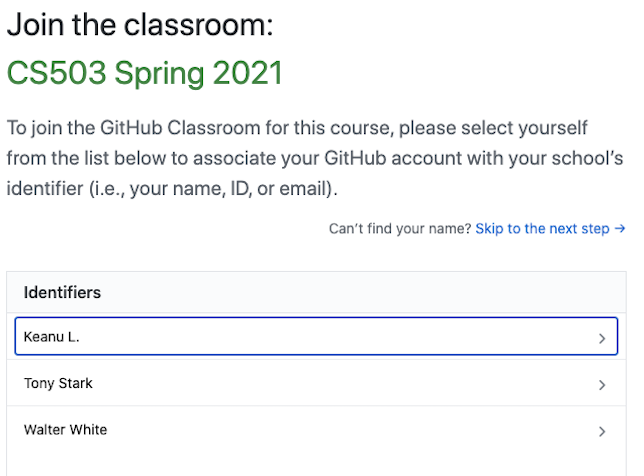
\includegraphics[height=5cm, frame]{img02}

  % \todo{Update github classroom link}
\item \textbf{Accept the assignment (Create a team).}
  Use the link provided in the Ed announcement to accept the assignment on GitHub Classroom.

  % \textbf{[TODO: Replace the link after the assignment is set up on Github Classroom]}

  The first person in a team accepting the assignment need to create a team. Please use your group name on Brightspace as your team name (e.g. Lab 2 - Group 1). Other team members should find and join the team. Please double-check the group name before you join.

  You should see screens similar to these:

  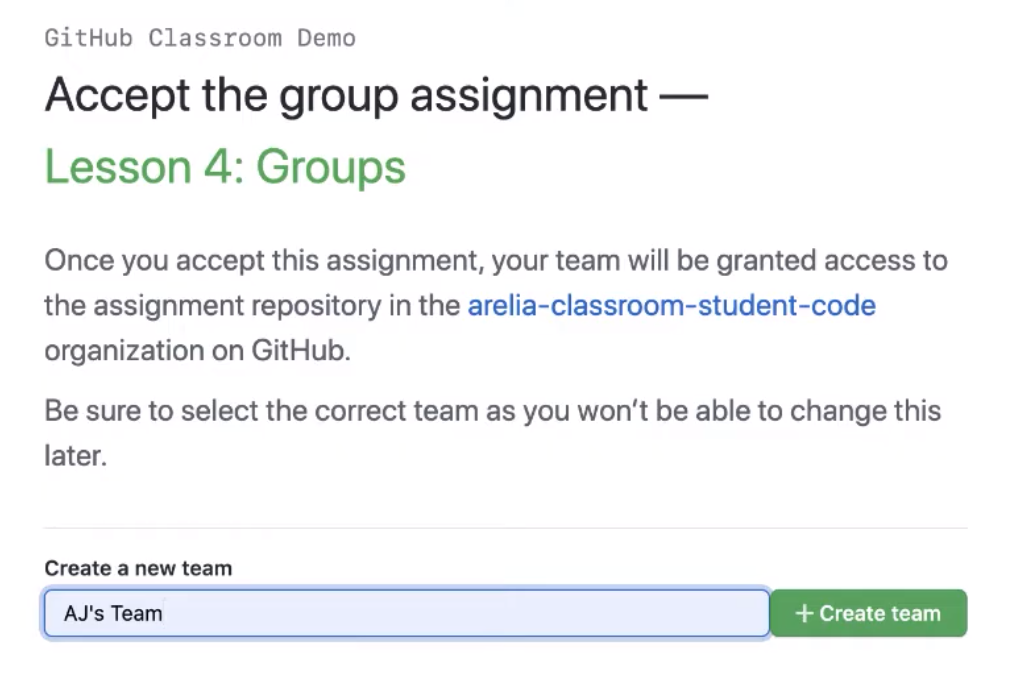
\includegraphics[height=5cm, frame]{img05}
  \hspace{1cm}
  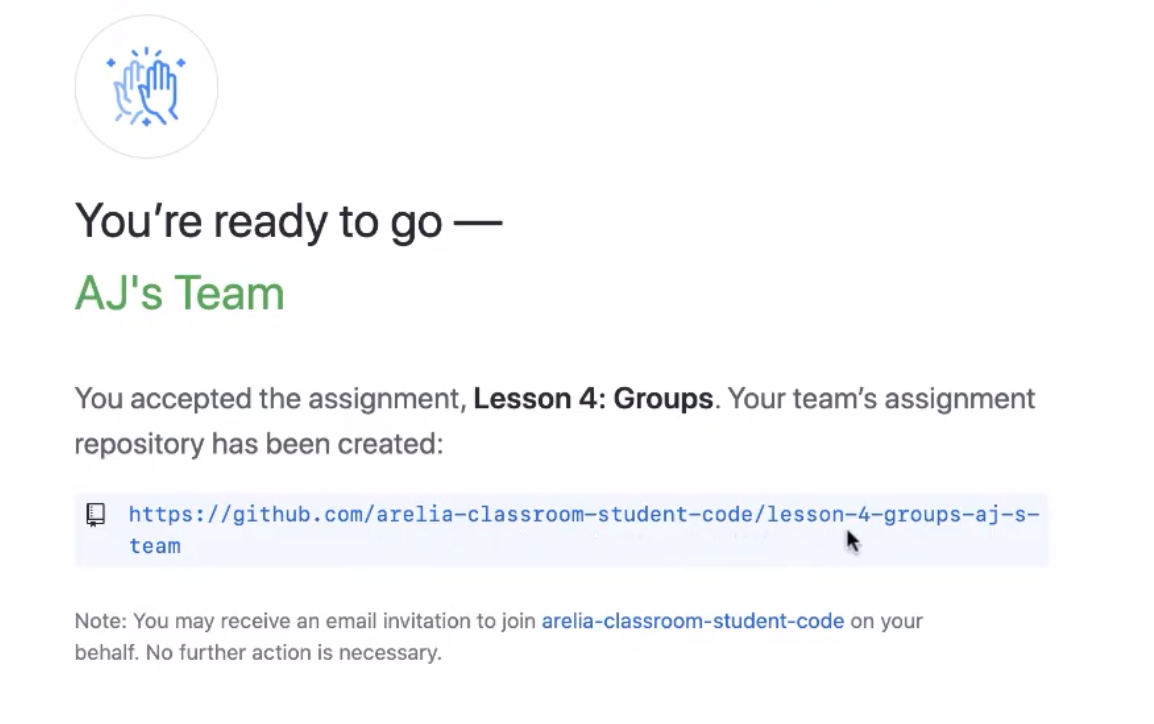
\includegraphics[height=5cm, frame]{img06}

\item \textbf{Accept the assignment (Join a team).}

You should see screens similar to these:

  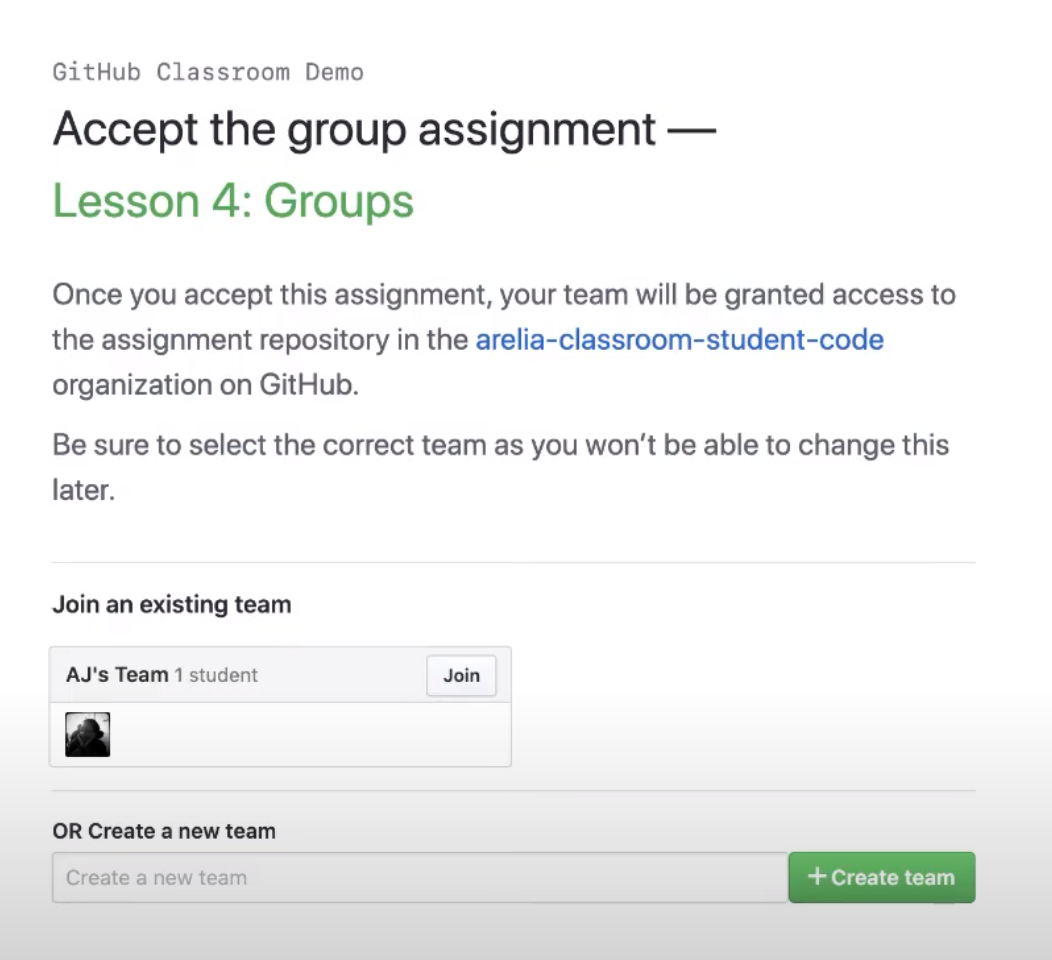
\includegraphics[height=5cm, frame]{img07}

Find your team and click join.

\item \textbf{Get you repo URL.}
  As the image shows, your project repository will have the
  format:\\
  \url{https://github.com/cs408-spring-2026/<projectName>-<yourTeamName>/}
\end{enumerate}

\subsection{Development workflow}
\label{development-workflow}

In case you forget the project repository name, you can go to
\url{https://github.com/cs408-spring-2026} to find it. For illustration
purposes, we will \textbf{assume} that your project is under
\emph{github.com/cs408-spring-2026/cs408-lab2-lab-2-group-1} and your team's name is
\textit{Lab 2 - Group 1}, so please adjust the links/directories accordingly.

\begin{enumerate}

\item \textbf{Clone the project repository.}

For example, to clone the repository in a new \textit{myclass} folder in your home
directory you should execute the following commands:

\begin{verbatim}
$ mkdir -p ~/myclass/; cd ~/myclass/;
$ git clone https://github.com/cs408-spring-2026/cs408-lab2-lab-2-group-1.git
$ cd lab-2-group-1/
\end{verbatim}

This project folder, \emph{lab-2-group-1}, would be your
project's \textbf{root directory}.

\item \textbf{Modify the source code as needed.}


% Note that in some cases (e.g., when adding new files) you need to run
% `make clean'`' before `make'  to reload header modifications, otherwise
% your build might be incomplete.

\item \textbf{Commit and push changes to the private GitHub server repo regularly.}

Note that you are required to regularly commit and push your changes to the private git
in GitHub Classrooms.

\begin{verbatim}
$ git commit
$ git push
\end{verbatim}

\end{enumerate}

\section*{References}

\noindent [1] Barton P. Miller, Louis Fredriksen, and Bryan So. 1990. An empirical study of the reliability of UNIX utilities. Com- munications of the ACM 33, 12 (1990), 32–44.


\noindent [2] Syzkaller. \url{https://github.com/google/syzkaller}

\noindent [3] Go Fuzzing. \url{https://go.dev/doc/security/fuzz/}

\noindent [4] Sanitizer Coverage \url{https://clang.llvm.org/docs/SanitizerCoverage.html}

\noindent [5] Aschermann et al. NAUTILUS: Fishing for Deep Bugs with Grammars. (NDSS '19) \url{https://www.ndss-symposium.org/wp-content/uploads/2019/02/ndss2019_04A-3_Aschermann_paper.pdf}

\noindent [6] AFLPlusPlus. \url{https://github.com/AFLplusplus/AFLplusplus/tree/stable}

\noindent [7] Fioraldi et al. LibAFL: A Framework to Build  Modular and Reusable Fuzzers. (CCS '22) \url{https://dl.acm.org/doi/pdf/10.1145/3548606.3560602}

%\newpage
%\bibliographystyle{abbrvnat}
%\bibliography{n-str,p,n}

\end{document}
